%#!latex
\documentclass[submit]{elex2024}%%submit option for submit

\usepackage{seqsplit}
\usepackage{multirow}
\usepackage{makecell}
\usepackage{graphicx}
\usepackage{threeparttable}
\let\uline\underline

\type{LETTER}

\title{An Energy-Efficient Digital Computing-In-Memory STT-MRAM Macro for AdderNets with Optimized Addition Operations}

\author{Yuan Xue}{1,2,3}[xueyuan@ime.ac.cn]
%\author{Xing Zhao}{1,2}[zhaoxing@ime.ac.cn]
\author{Sinan Zou}{1,2,3}[zousinan@ime.ac.cn]
\author{Jianfeng Gao}{1,2}[gaojianfegn@ime.ac.cn]
\author{Yilu Li}{1,2}[liyilu@ime.ac.cn]<2481216>%%% 1324567 ieice membership,  0000-0000-0000-0000 orcid
\author{Yan Cui*}{1,2}[cuiyan@ime.ac.cn]
\author{Jun Luo*}{1,2,3}[luojun@ime.ac.cn]

\affiliate{1}{Key Laboratory of Fabrication Technologies for Integrated Circuits, Chinese Academy of Sciences, Beijing 100029}
\affiliate{2}{Institute of Microelectronics, Chinese Academy of Sciences (IMECAS), Beijing 100029, China}
\affiliate{3}{University of Chinese Academy of Sciences (UCAS), Beijing 100049, China}

\vol{}
\no{}


%\doi{10.1587/elex.XX.XXXXXXXX}
%\received{2024/10/10}
%\accepted{2024/10/10}
%\publicized{2024/12/31}
\copyedited{2025/1/29}


\setcounter{page}{1}

\begin{document}

\maketitle 

\begin{abstract}
Adder neural networks (AdderNets), a promising lightweight alternative to traditional CNNs, face the "memory wall" challenge in von-Neumann architectures. Computing-in-memory (CIM) has emerged as a promising solution to address this memory bottleneck. This work proposes a novel spin-transfer torque magnetic random-access memory based digital-CIM macro tailored for AdderNets mapping, leveraging Boolean logic-optimized architecture to seamlessly integrate storage and computation. The architecture is validated through simulations under 40 nm CMOS technology. Results show that the architecture achieves an energy efficiency of 31.48 TOPS/W in 8-bit network inference, representing a 1.5$\times$ to 4.1$\times$ improvement over state-of-the-art digital CIM designs.
\end{abstract}

\begin{keywords}
Computing-in-memory (CIM), digital computing, magnetic random-access memory (MRAM), adder neural network
\end{keywords}

\begin{classification}
Integrated circuits (logic)
\end{classification}


\section{Introduction}

Convolutional neural networks (CNNs) represent a classic paradigm of generative artificial networks and are widely applied across various domains, including artificial intelligence and the Internet of Things (IoT). Learning algorithms based on multiply-accumulate (MAC) operations have dominated and driven the rapid development of high-performance computing~\cite{1,2,3}. Currently, most mainstream neural networks are deployed on computational systems based on the von-Neumann architecture. These platforms process and store intermediate data and weight information generated during network calculation. The intensive data transfer between processors and storage units results in significant latency and energy costs~\cite{4}, leading to a performance bottleneck commonly known as the “memory wall”~\cite{5}. This severely limits the integration of neural networks in resource-constrained devices, which is critical for embedded and edge applications~\cite{6,7}. \\
Computing-in-memory (CIM) has emerged as a promising approach to mitigate this challenge. It directly deploys partial computational tasks to memory cells, physically eliminating the boundary between processors and memory units~\cite{8,9}. As the architectural cornerstone of CIM systems, the intrinsic properties of memory cells dictate system performance~\cite{10}. Neuromorphic implementations exploit their programmable conductance to emulate synaptic functions and enable logic-in-memory operations~\cite{11}. Spin-transfer torque (STT) and spin-orbit torque (SOT) based magnetic random-access memory (MRAM) utilizes crossbar arrays for parallel computation, demonstrating superior energy efficiency and performance over conventional CMOS-based in-memory computing (IMC) designs~\cite{12,13,14,15,16}.\\
Adder neural networks (AdderNets), a novel type of CNNs, replaces multiplication operations with addition in convolution operations to reduce computational complexity~\cite{17}. AdderNets utilize the $\ell_1$-distance instead of the L2 norm to measure feature-filter discrepancies, demonstrating competitive performance in tasks such as computer vision~\cite{18}, object detection~\cite{19}, and super-resolution~\cite{20}. A hardware-algorithm co-design methodology has facilitated successful AdderNet implementations on multiple digital CIM platforms, including SRAM~\cite{21}, FPGA~\cite{22}, and MRAM~\cite{23}. However, these digital IMC schemes inevitably rely on dedicated auxiliary processing units (e.g., adder trees or multi-stage latches) for intermediate data storage and $\ell_1$ -distance computation. Such architectures inherently limit advancements in computational parallelism and efficiency. \\
In this paper, we present a novel STT-MRAM-based digital CIM macro designed for high-performance and energy-efficient inference in AdderNets. Our macro integrates comprehensive basic Boolean logic operations tailored for the accelerator architecture of AdderNets, along with an efficient $\ell_1$-distance computation method. The main contributions of this paper can be summarized as follows: (1) We propose an efficient IMC paradigm tailored for low bit-width AdderNet training, which replaces the convolution process with the  $\ell_1$-distance of vectors to reduce computational cost. (2) We introduce an innovative method for co-optimizing architecture and circuits based on Boolean logic, achieving seamless integration of storage functions and logical computation operations within the MRAM array. (3) We validate the proposed CIM architecture through simulations under SMIC 40 nm CMOS technology. Results demonstrate that our additive logic implementation achieves over 3.6$\times$ energy consumption optimization. Additionally, in 8-bit network inference, the architecture delivers a maximum energy efficiency of 31.48 TOPS/W. 

\section{Computing in STT-MRAM fundamentals}

\subsection{2T1MTJ Bit-cell}
A typical STT-MRAM cell consists of magnetic tunnel junctions (MTJs) and one or more access transistors~\cite{24}. The core of the MTJ is a sandwich structure formed by two ferromagnetic metal layers separated by a barrier layer, commonly made of MgO. The two ferromagnetic layers are distinguished as the reference layer (RL) and the free layer (FL) based on the difficulty of magnetization flipping. Depending on the magnetization orientations of the RL and FL, the MTJ can exhibit high-resistance (AP) or low-resistance (P) states~\cite{25}. Accordingly, we define the AP and P states of the MTJ as representing logical `1' and `0', respectively.
\begin{figure}[htb]
    \centering
    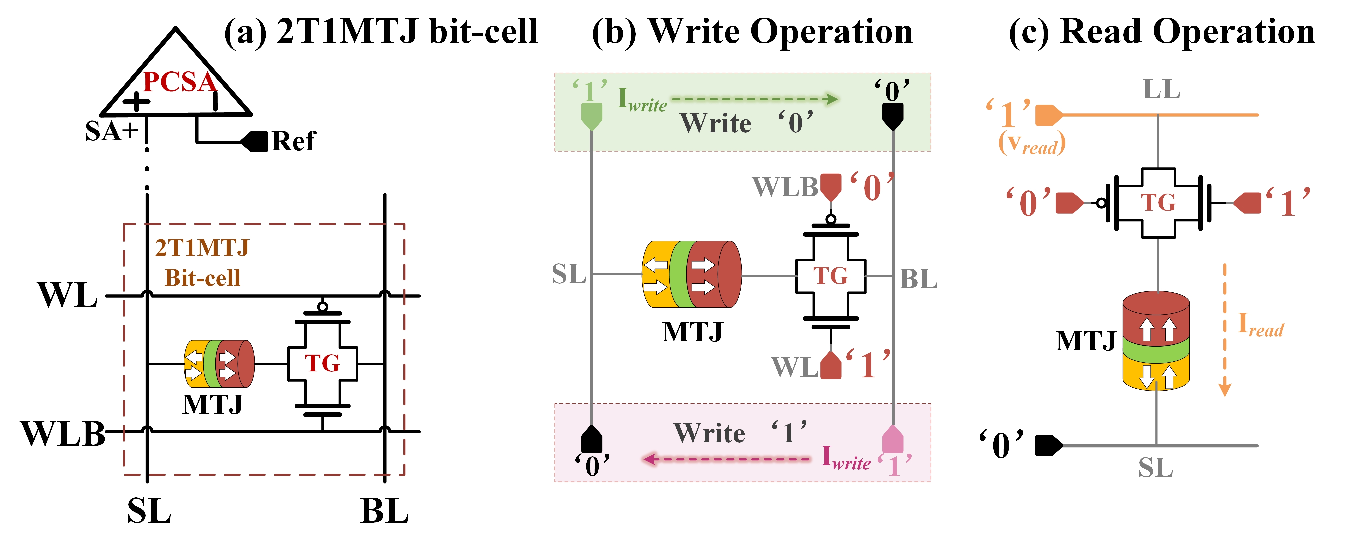
\includegraphics[width=8cm]{Figures/fig1.pdf}
    \caption{(a) Structure of the Proposed 2T1MTJ Bitcell with (b) Write and (c) Read operations.}
    \label{fig:1}
\end{figure}

\noindent
We use a 2T-1MTJ bit-cell structure that enhances storage density while also handling logic computation tasks. Fig.~\ref{fig:1} illustrates the actual configuration: a single MTJ is accessed and interconnected through one transmission gate (TG). During write operations, the TG is activated by the word lines (WLs) to generate the write current Iwrite, with the direction and magnitude of the current determined by the voltage difference applied between the source line (SL) and the bit line (BL). For read operations, the target cell will connecting the cell to the readout circuit, which is mainly composed of a pre-charge current sense amplifier (PCSA).
\begin{table}[ht]
    \small
    \caption{Key parameters of the perpendicular-magnetic-anisotropy MTJ.} 
    \label{tab:1}
    \centering
    \tabcolsep.2\tabcolsep
    \begin{tabular}{ccccc}
    \hline
    \textbf{Parameter}      & \quad & \textbf{Description}                           & \quad & \textbf{Value}  \\
    \hline
    Area      			    & \quad & MTJ surface (W x L)                     & \quad & 32 nm x 32 nm        \\
    \hline
    tox    				    & \quad & Thickness of the Oxide Barrier                 & \quad & 0.85 nm        \\
    \hline
    tsl                     & \quad & Thickness of the Free Layer                    & \quad & 1.3 nm       \\
    \hline
    TMR                     & \quad & TMR (0) with Zero Volt Bias Voltage            & \quad & 200$\%$      \\
    \hline
    $T_0$                   & \quad & Ambient Temperature                            & \quad & 300 K        \\
    \hline
    $I_{c0}$     			& \quad & Critical Switching Current                     & \quad & 34.1 µA        \\
    \hline
    $R_{MTJ}$      			& \quad & Nominal Resistance at $R_L$ ($R_H$) of MTJ     & \quad & 6.3 $K\Omega$ (18.9 $K\Omega$)        \\
    \hline
    \end{tabular}
\end{table}

\noindent
A Verilog-A compact model~\cite{26} describes the perpendicular-magnetic-anisotropy MTJs (pMTJs) device. Its critical parameters are shown in Table~\ref{tab:1}, which are based on theoretical calculation and experimental measurements~\cite{27}. For the access transistors, a commercial 40 nm CMOS technology was considered.
\begin{figure}[htb]
    \centering
    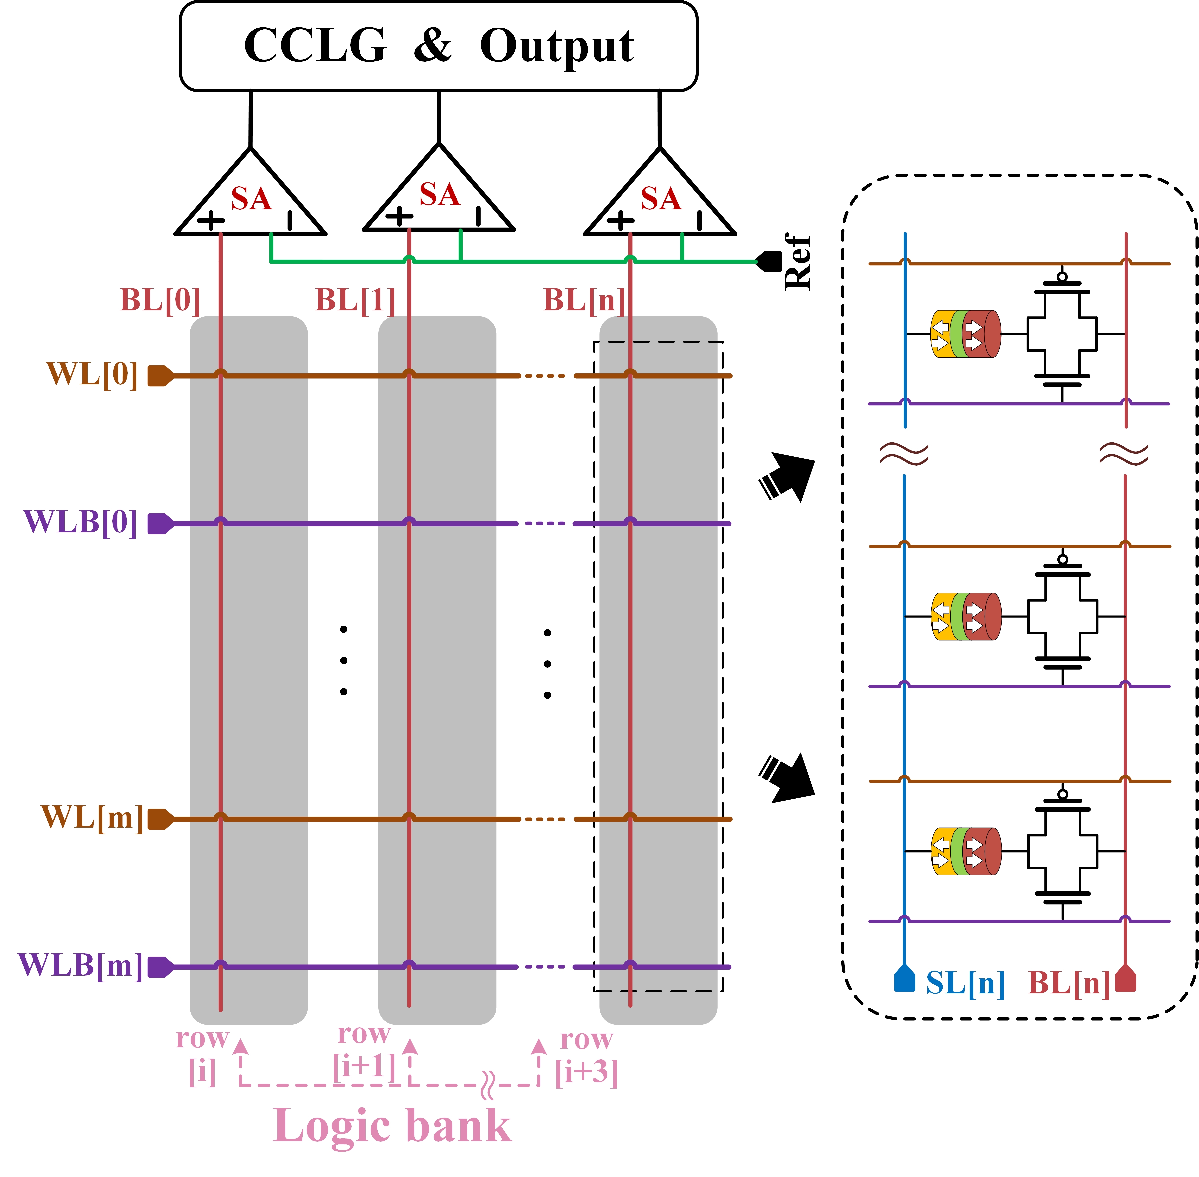
\includegraphics[width=6cm]{Figures/fig2.pdf}
    \caption{Proposed memory array architecture for enhanced logic computations.}
    \label{fig:2}
\end{figure}
\begin{figure}[htb]
    \begin{center}
    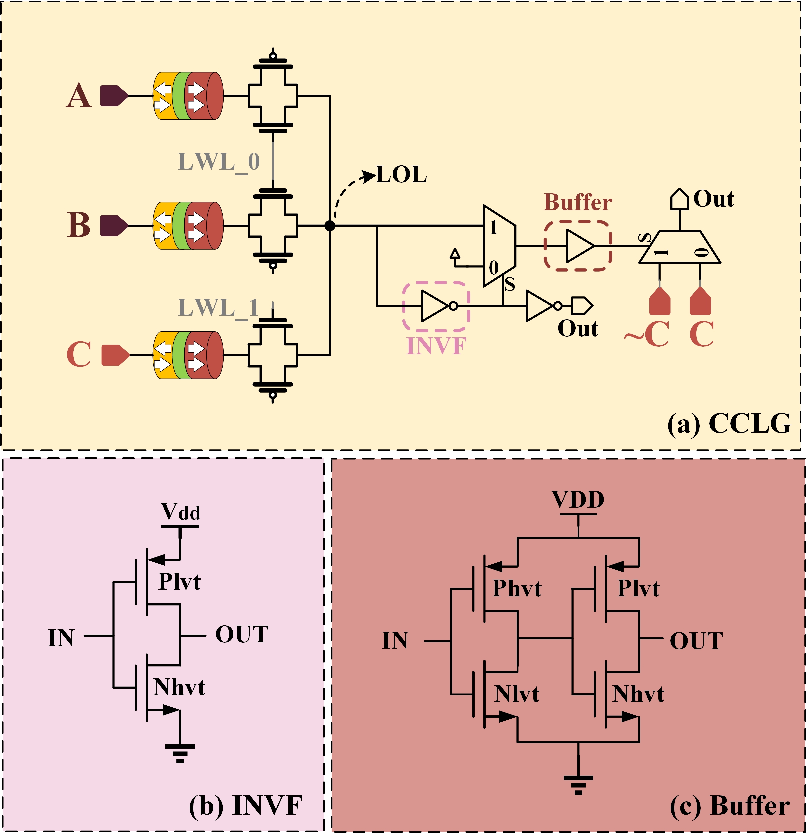
\includegraphics[width=6cm]{Figures/fig3.pdf}
    \end{center}
    \caption{(a) Overview of the proposed configurable composite logic gate (CCLG) and its components: (b) INVF and (c) Buffer.}
    \label{fig:3}
\end{figure}
\begin{table}[ht]
    \centering
    \caption{Configuring logic gates for diverse logical operations}
    \label{tab:2}
    \begin{tabular}{|c|c|c|c|}
    \hline
    \textbf{Signals} & \textbf{Input} & \textbf{Description} & \textbf{Operations} \\
    \hline
    \multirow{9}{*}{\centering \makecell[l]{LWL\_1=1 \\ LWL\_2=1}} 
     & A & Input & \multirow{3}{*}{AND/NAND} \\ \cline{2-3}
     & B & Input & \\ \cline{2-3}
     & C & '0' & \\ \cline{2-4}
    \cline{2-3}
     & A & Input & \multirow{3}{*}{OR/NOR} \\ \cline{2-3}
     & B & Input & \\ \cline{2-3}
     & C & '1' & \\ \cline{2-4}
    \cline{2-3}
     & A & Input & \multirow{3}{*}{MAJ/MNJ} \\ \cline{2-3}
     & B & Input & \\ \cline{2-3}
     & C & Input & \\ \hline
    
    \multirow{3}{*}{\centering \makecell[l]{LWL\_1=1 \\ LWL\_2=0}} 
     & A & Input & \multirow{3}{*}{XOR/XNOR} \\ \cline{2-3}
     & B & Input & \\ \cline{2-3}
     & C & X & \\ \hline
    \end{tabular}
\end{table}
\subsection{Motivation for in-memory logic based on readout circuit}
Fig.~\ref{fig:2} illustrates the proposed 2T1M bit-cell, which implements inter-row Boolean logic through a sense amplifier (SA) and a configurable composite logic gate (CCLG). The NVM array is divided into logic banks, each containing three columns connected to the CCLG via the SA. The first three columns form a majority gate for basic Boolean logic, while the fourth column serves as a redundancy line for data storage or composite logic. \\
As shown in Fig.~\ref{fig:3}(a), external control signals in the CCLG enable switching between different logic operations. Table~\ref{tab:2} summarizes the signal configurations and corresponding logic functions. For basic Boolean and MAJ operations, ports $A$, $B$, and $C$ are connected via TG, while port $D$ is isolated. Port $C$ is set to `0' for AND/NAND, `1' for OR/NOR, or $\text{MAJ/MNJ}(A, B, C)$. For XOR/XNOR, ports $C$ and $D$ are isolated, and the SA reads operands $A$ and $B$, triggering a voltage change at the logic output line (LOL). This change is captured by a feedback structure (INV and MUXs) and amplified for output. Fig.~\ref{fig:3}(b) and Fig.~\ref{fig:3}(c) detail the feedback circuit, which utilizes multi-threshold voltage transistors to fine-tune the logic output margin. 
\subsection{Full Adder for CIM}
In the realm of CIM, the Full Adder (FA) serves as a crucial hardware unit for performing addition and multiplication operations. It is typically realized using specific CMOS combinational logic circuits or digital/analog NVM units combined with sequential logic scheduling~\cite{13,16,28}. To balance computational efficiency and throughput, we propose an innovative high-parallel full addition solution based on CCLG, as illustrated in Fig.~\ref{fig:4}.
\begin{figure}[htb]
    \begin{center}
    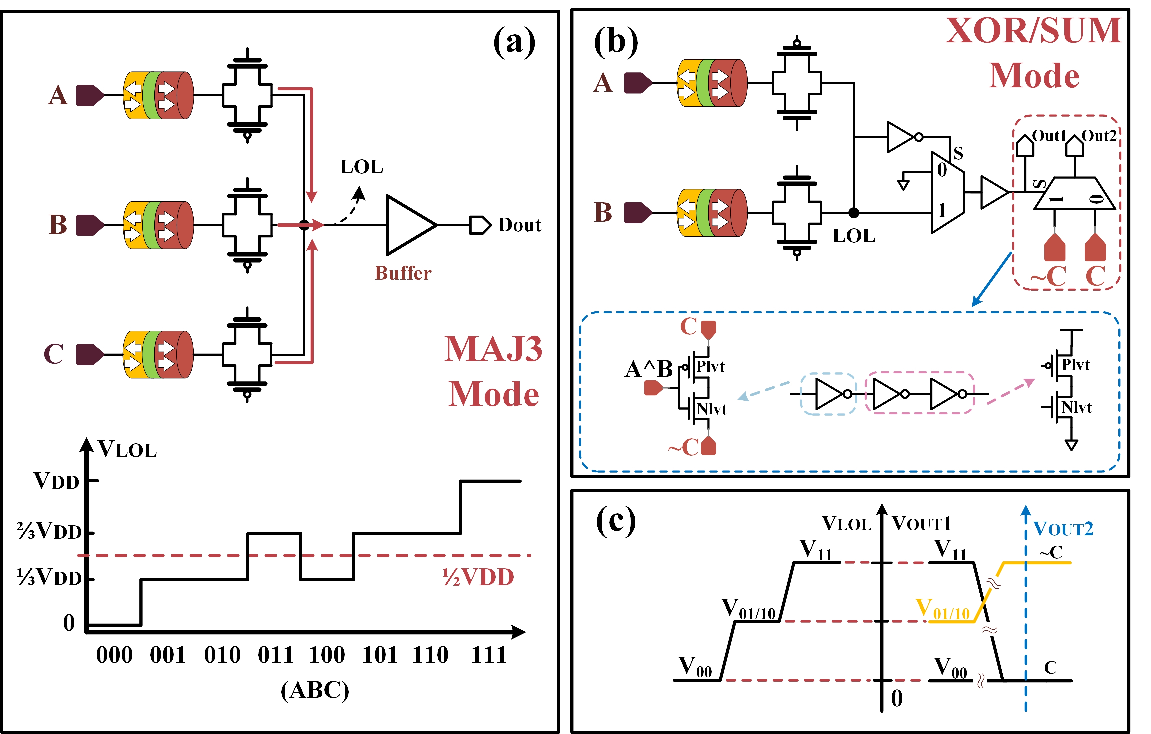
\includegraphics[width=8cm]{Figures/fig4.pdf}
    \end{center}
    \caption{(a) Resistive-based MAJ3 gate. (b) Proposed feedback-selective XOR/SUM logic gate circuit structure, and (c) Its node voltage distribution.}
    \label{fig:4}
\end{figure}

\noindent
Generally, the input of the FA consists of two computational input bits, $A$ and $B$, along with a carry-in bit ($C_i$). The FA generates and outputs the sum ($S$) and the carry-out ($C_{i+1}$) based on the logical relationships described in Eq.~\ref{eq1}: 
\begin{equation}
    \begin{aligned}
        C_{i+1} = AB + &\left( A \oplus B \right) C_i = AB + AC_i + BC_i \\
        &S = A \oplus B \oplus C_i
        \label{eq1}
    \end{aligned}
\end{equation}
It is important to note that Eq.~\ref{eq1} can be equivalently expressed as Eq.~\ref{eq2}:
\begin{equation}
    C_{out} = M_3\left(A,B,C_{in}\right)
    \label{eq2}
\end{equation}%
Therefore, we configure the CCLG to operate in MAJ3 logic mode, as shown in Fig.~\ref{fig:3}(a). Using Eq.~\ref{eq2}, the carry value $C_i$ for each bit of input data $A$ and $B$ is iteratively generated. Additionally, we introduce a decision mechanism as follows: 
\begin{equation}
\begin{aligned}
    S &=    (A\oplus B)\oplus C\\
      &=    SEL(\bar{C},C)|_{A\oplus B}
    \label{eq3}
\end{aligned}
\end{equation}%
We configure the CCLG to operate in XOR logic mode, and its topology is shown in Fig.~\ref{fig:4}(b). At this stage, the voltages at the LOL node and Out1 vary according to the level signals at ports $A$ and $B$. Based on the logic of Eq.~\ref{eq3}, the final sum value is computed at Out2. The voltage waveforms at each node are shown in Fig.~\ref{fig:4}(c). 

\begin{figure}[htb]
    \begin{center}
    \includegraphics[width=8cm]{Figures/fig5.pdf}
    \end{center}
    \caption{Overall architecture of the proposed CIM macro. (a) Circuit-level interconnection design of the NVM array. (b) Write driver used for multi-functional switching and (c) Its waveforms in different function mode.}
    \label{fig:5}
\end{figure}
\section{Hardware implementation strategies for CIM framework}
AdderNets introduce a novel approach by replacing traditional multiplicative convolutions with additive convolutions. This innovation significantly reduces computational energy while maintaining high inference accuracy. Such advancements enhance the feasibility of deploying neural networks on edge devices and hardware platforms~\cite{29}.
\begin{equation}
    \begin{aligned}
        Y=-\sum_{i=0}^{d}\sum_{j=0}^{d}\sum_{k=0}^{C_{in}}\left|X\left(m+i,n+j,k\right)-W\left(i,j,k,t\right)\right|
    \label{eq4}
    \end{aligned}
\end{equation}
The core concept of AdderNets is to use the $\ell_1$-distance metric to measure the similarity between the input feature $X$ and the filters $W$, as shown in Eq.~\ref{eq4}. This approach eliminates the need for complex multiplications typically required for traditional Euclidean distance calculations, significantly reducing computational complexity and energy consumption.
\subsection{CIM macro description} 
To demonstrate the hardware implementation of the proposed additive convolution, we employ an $m \times n$ MRAM array. As shown in Fig.\ref{fig:5}(a), the array comprises $m \times n$ cells, each with a 2T1MTJ structure. Fig.~\ref{fig:5}(b) and (c) illustrates the write driver design and its waveforms in different operational modes. This architecture enables independent and parallel writing to each column's computing unit via dedicated write drivers, while read operations and logical processing are performed in parallel across rows.
\begin{figure}[htb]
    \begin{center}
    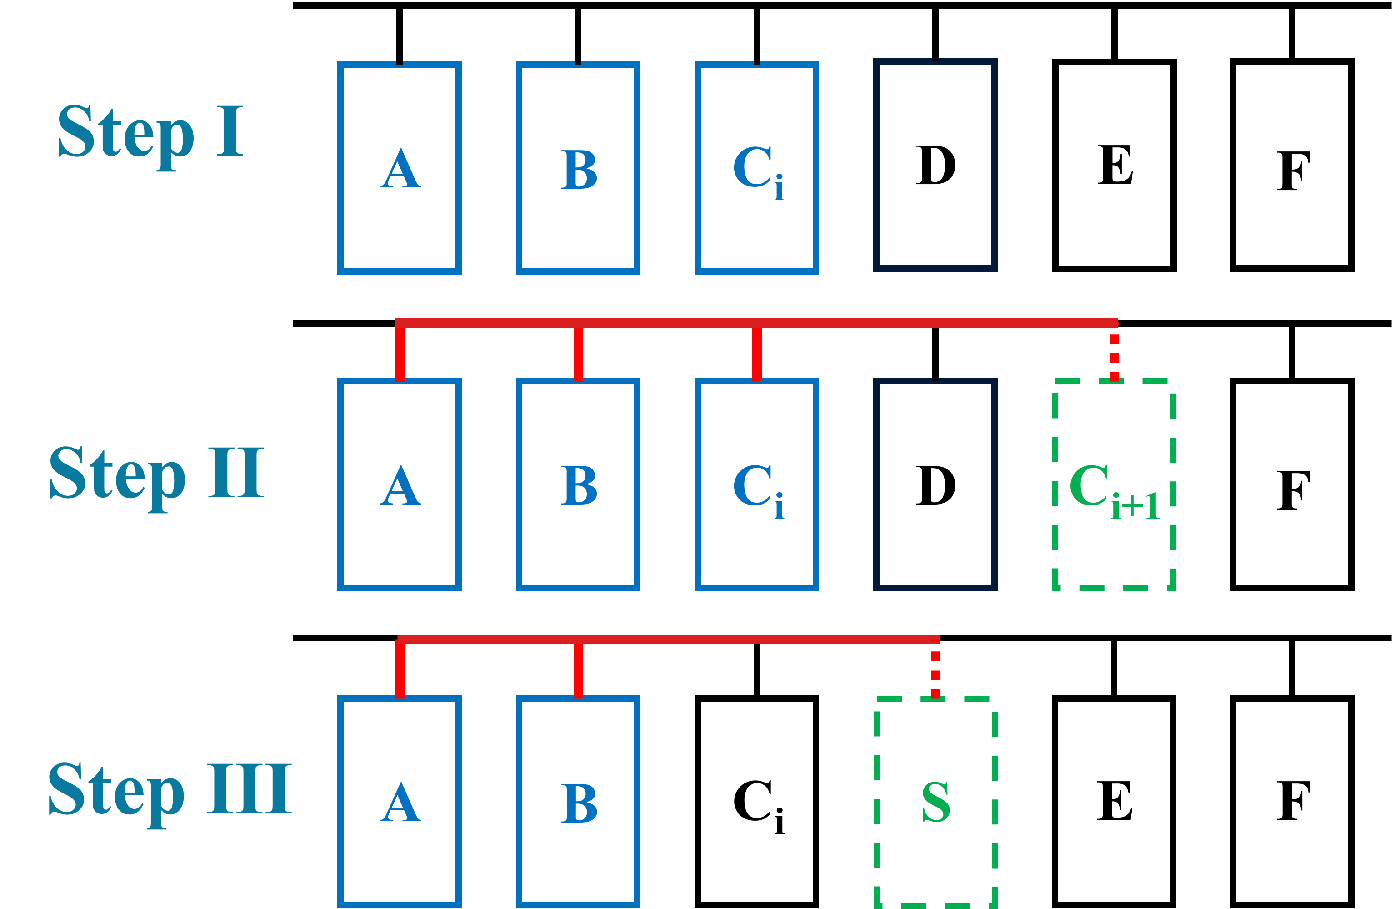
\includegraphics[width=7cm]{Figures/fig6.pdf}
    \end{center}
    \caption{Illustration of the array-level implementation scheme for a single-bit full adder.}
    \label{fig:6}
\end{figure}
\begin{figure}[htb]
    \centering
    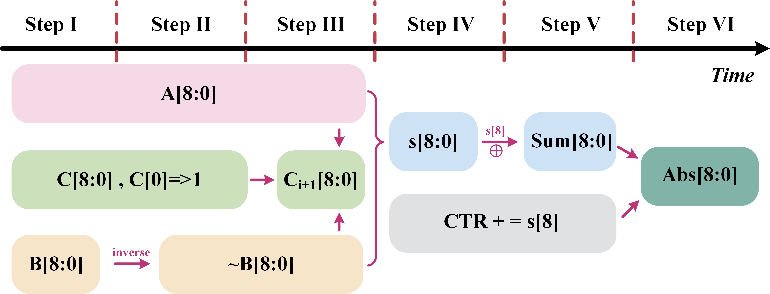
\includegraphics[width=7cm]{Figures/fig7.pdf}
    \caption{Illustration of the step-by-step operations for implementing an 8-bit metric function S based on the proposed architecture.}
    \label{fig:7}
\end{figure}
\subsection{Full adder design} 
To execute the additive convolution mapping, it is essential to establish a FA circuit. Fig.~\ref{fig:6} illustrates the construction process of a single-bit adder.
$Step 1$: We initialize all MTJ units to the state '0'. Load operands $A$ and $B$, and the carry-in signal $C_i$, from external registers into their corresponding MTJ cells. 
$Step 2$: Adjust the control signals to place the array in read mode and configure the CCLG to enter MAJ logic state. Perform MAJ logic on the first three cols of MTJ cells storing operands $A$, $B$, and $C_i$. The carry-out signal Ci+1 is calculated according to Eq.~\ref{eq2}.
$Step 3$: Reconfigure the RCLG to enter XOR logic state. Execute XOR logic on the top two cols of MTJ cells storing operands $A$ and $B$, yielding an intermediate result $(A\oplus B)$. The final sum, $S$, is then determined using Eq.~\ref{eq3} and stored.


\noindent
Fig.~\ref{fig:7} illustrates the construction process of the multi-bit FA. To FA operations for multi-bit data, the ripple carry adder (RCA) principle is employed, which propagates carry signals to enable computation~\cite{30}. In hardware implementations, the $\ell_1$-distance calculation, defined as the sum of absolute differences between two vectors, is optimized using two's complement arithmetic to convert subtractions into additions~\cite{31}. To balance computational precision and energy efficiency, an 8-bit quantization scheme is adopted for the design of digital computing architectures~\cite{32}. \\
Furthermore, to implement the absolute value operation, we need to evaluate the sign bit s[8]: when s[8]==1, the sum value s[8:0] needs to be bit-wise inverted and incremented by 1; conversely, when s[8]==0, the sum value can be output directly without any processing. This evaluation process can be expressed by the Eq.~\ref{eq5}:
\begin{equation}
    \begin{aligned}
        Sum[i] &=    s[8]\oplus s[i]\\
        Abs    &=   Sum + s[8]
        \label{eq5}
    \end{aligned}
\end{equation} 

\section{Design methodology $\&$ performance evaluation}
To evaluate the performance of the proposed computing architecture, we utilized the SMIC 40 nm commercial PDK library for simulating hybrid CMOS/MTJ circuits. Using the Cadence 
\begin{table}[ht]
    \small
    \caption{Bit-cell level evaluation in memory operations.} 
    \label{tab:3}
    \centering
    \tabcolsep.2\tabcolsep
    \begin{tabular}{lccccccccccc}
    \hline
    \textbf{Oper.}     & \quad & \textbf{Iwrite (uA)}     & \quad & \textbf{Vwrite (mV)}         & \quad & \textbf{t (ns)}       & \quad & \textbf{PDP (fJ)}        & \quad & \textbf{Iw/Ic0}             \\
    \hline
    \textbf{Write 0}      	& \quad & 119.8                    & \quad & 967.7                        & \quad & 1.76                  & \quad & 207.5                    & \quad & 2.48              \\
    \hline
    \textbf{Write 1}    	& \quad & 130.2                    & \quad & 821.8                        & \quad & 1.46                  & \quad & 156.2                    & \quad & 2.96     \\
    \hline
    \textbf{Oper.}     & \quad & \textbf{Iread (uA)}      & \quad & \textbf{Vread (mV)}  & \quad & \textbf{Delay (ns)}  & \quad & \textbf{Power (fJ)}   & \quad & \textbf{Error ($\%$)}     \\
    \hline
    \textbf{Read 0}         & \quad & 9.310                    & \quad & 58.78                & \quad & 1.0                  & \quad & 0.547                 & \quad & 0.3                            \\
    \hline
    \textbf{Read 1}         & \quad & 6.101                    & \quad & 81.25                & \quad & 1.0                   & \quad & 0.496                 & \quad & 2                              \\
    \hline
    \end{tabular}
\end{table}
\begin{table}[ht]
    \small
    \caption{Evaluation of the proposed CCLG in different logic mode.} 
    \label{tab:4}
    \centering
    \tabcolsep.4\tabcolsep
    \begin{tabular}{lcccccccc}
    \hline
    \textbf{Evaluation}     & \quad & \textbf{OR/NOR}     & \quad & \textbf{AND/NAND}       & \quad & \textbf{XOR/XNOR}      & \quad & \textbf{MAJ/MNJ}       \\
    \hline
    \textbf{Power (uW)}     & \quad & 5.867               & \quad & 4.983                   & \quad & 3.088                  & \quad & 4.581                  \\
    \hline
    \textbf{Delay (ps)}    	& \quad & 65.02               & \quad & 39.95                   & \quad & 63.98                  & \quad & 48.79                  \\
    \hline
    \textbf{PDP (aJ)}       & \quad & 381.5               & \quad & 199.1                   & \quad & 197.6                  & \quad & 223.5                  \\
    \hline
    \end{tabular}
\end{table}
Virtuoso IC6.1.8 environment, we employed Virtuoso ADEL and Spectre tools to construct and evaluate the circuit structures. Additionally, we performed circuit-level performance simulations using the NeuroSim Framework~\cite{33}. 

\subsection{MRAM bit-cell design and simulation}

To enhance the accuracy of computational results, ensuring the high reliability of the MTJ's read and write processes is crucial. While increasing the write pulse current to enhance write reliability, we also introduce a PCSA structure to balance power consumption and accuracy during the readout process~\cite{34}. Under the framework of the Verilog-A pMTJs model used, our read and write pulse times are set to 1 ns and 2 ns, respectively. Operating at 1.1 V, the details during the read and write processes are presented in Table~\ref{tab:3}.

\subsection{Circuit-level simulation of the proposed CCLG}
The proposed CCLG structure's basic logic functionality was tested using 1,000 times Monte Carlo (MC) simulations, evaluating key parameters like delay and power consumption. Simulation results are shown in Fig.~\ref{fig:8}, with average values from the MC simulations detailed in Table~\ref{tab:4}.

\begin{figure}[htb]
    \begin{center}
    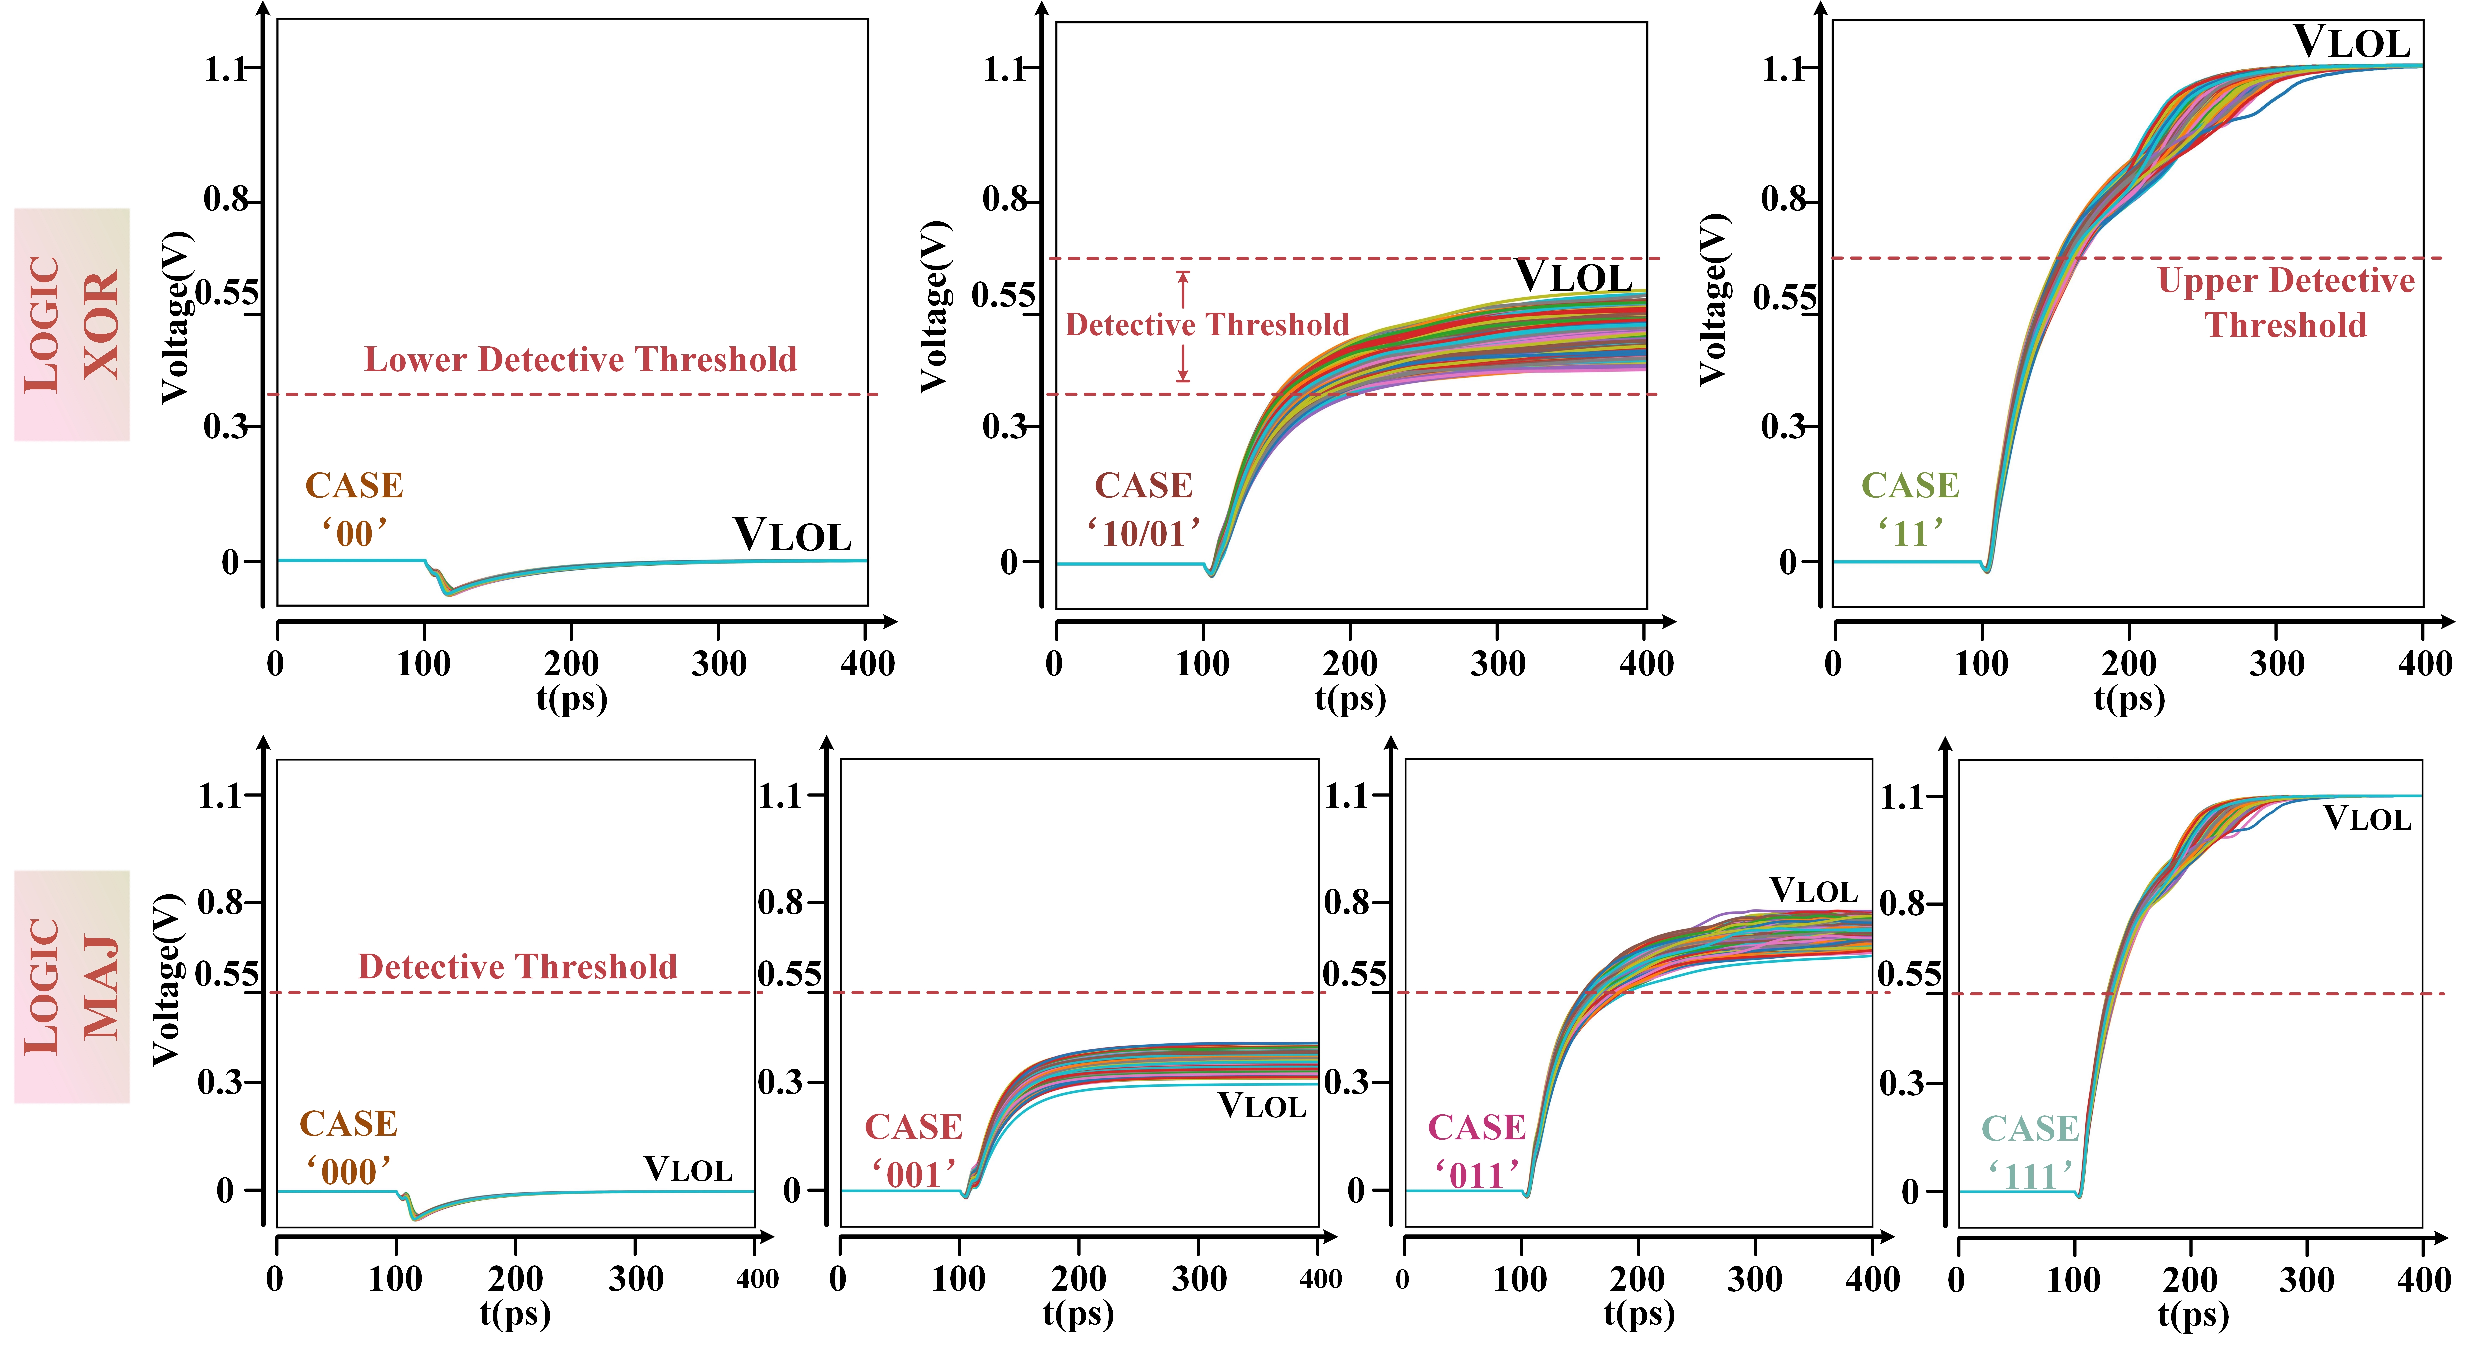
\includegraphics[width=8cm]{Figures/fig8.pdf}
    \end{center}
    \caption{MC simulation of proposed CCLG in different logic mode.}
    \label{fig:8}
\end{figure}
\subsection{Function simulation of addition operation}

Fig.~\ref{fig:9} illustrates the transient simulation waveforms of the $\ell_1$-distance calculation process. The activation value X = 47 and the weight W = 100 were used in the computation. During the initial clock cycle, the two's complement data corresponding to the activation X (X[8:0] = 0,0010,1111) and the weight W (W[8:0] = 0,0110,0100) were initialized in the same row of the array. Additionally, the carry data C[8:0] = 0,0000,0001 was also initialized. Subsequently, the carry data C[8:1] was computed bitwise according to Eq.~\ref{eq3}, and the updated carry data C[8:0] = 0,0011,1111 was written into the array within a single write cycle. Next, the sum value S[8:0] = 1,1100,1011 was computed in parallel according to Eq.~\ref{eq4}, and both the sum value and the sign bit S[8] = 1 were written into a new column. Finally, the absolute value A[8:0] = 0,00110100 was computed according to Eq.~\ref{eq5}, and the accumulation signal CTR = 1 was recorded. \\
The entire 8-bit $\ell_1$-distance computation process requires 31 ns, with the first 28 ns dedicated to the 8-bit two's complement addition of (A - W), consuming approximately 2.71 pJ. The final 3 ns are used to compute and output the absolute value result A[8:0] and the counter signal CTR, consuming approximately 1.72 pJ.

\begin{figure}[htb]
    \begin{center}
    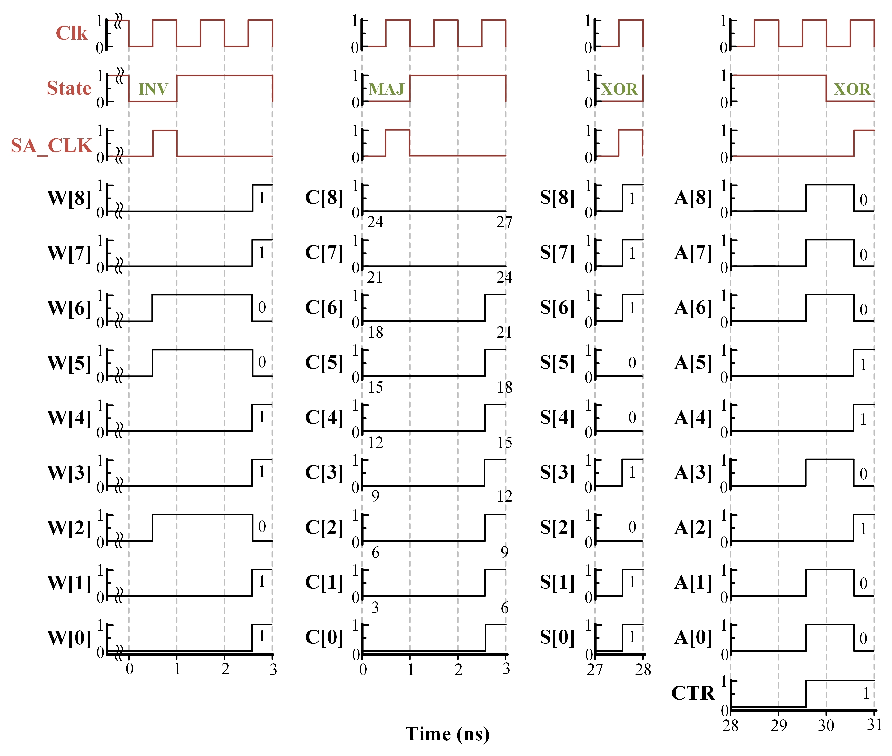
\includegraphics[width=7cm]{Figures/fig9.pdf}
    \end{center}
    \caption{Simulation waveforms during the absolute value calculation.}
    \label{fig:9}
\end{figure}
\begin{figure}[htb]
    \begin{center}
    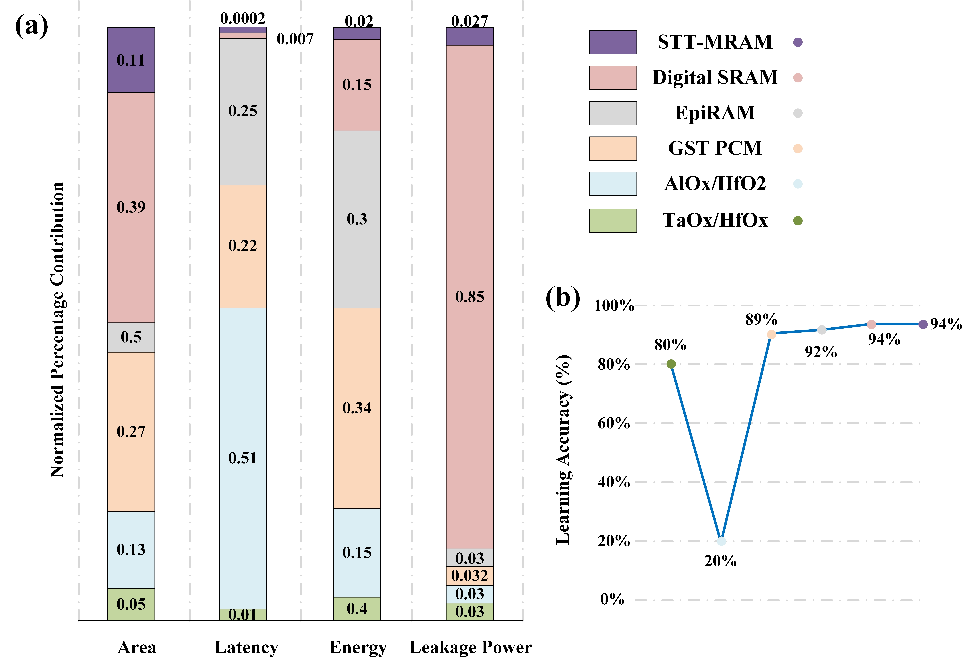
\includegraphics[width=7cm]{Figures/fig10.pdf}
    \end{center}
    \caption{(a) Normalized performance evaluation of different benchmark CIM frameworks and the proposed design. (b) Simulation learning accuracy comparison between our structure and others.}
    \label{fig:10}
\end{figure}
\begin{table}[ht]
    \centering
    \begin{threeparttable}
    \tabcolsep.6\tabcolsep
    \caption{Performance summary and comparison with related works}
    \label{tab:5}
    \begin{tabular}{|c|c|c|c|c|c|}
    \hline
    \quad                   &\textbf{[29]} & \textbf{[35]} & \textbf{[36]} & \textbf{[37]} & \makecell[c]{\textbf{This} \\ \textbf{Work}} \\
    \hline
    \textbf{Device}         & CPU & \makecell[c]{STT \\ MTJ} & \makecell[c]{SOT \\ MTJ} & \makecell[c]{SHE \\ MTJ} & \makecell[c]{STT \\ MTJ} \\
    \hline
    \textbf{Technology}     & 45 nm & 28 nm & 28 nm & 40 nm & 40 nm \\ 
    \hline
    \makecell[c]{\textbf{Cell} \\ \textbf{Structure}} & 46xT & \makecell[c]{8NVFF- \\ 8NVFA* } & \makecell[c]{256x32 \\ 2T1M } & \makecell[c]{7x8 \\ 2T1M } & \makecell[c]{3x8 \\ 2T1M } \\ 
    \hline
    \makecell[c]{\textbf{Computing} \\ \textbf{Type}} & \makecell[c]{8bit \\ RCA } & \makecell[c]{8bit \\ RCA } & \makecell[c]{8bit \\ PPA* } & \makecell[c]{8bit \\ RCA } & \makecell[c]{8bit \\ RCA } \\ 
    \hline
    \textbf{Latency (ns)}   & ~12 & 140 & 33.5 & 85 & ~28 \\ 
    \hline
    \textbf{Energy (pJ)}    & 70 & 50.93 & 51.6 & 10.65 & ~2.92 \\ 
    \hline
    \textbf{Voltage (V)}    & 1.1 & 0.7 & 1.2 & N/A & 1.1 \\ 
    \hline
    \end{tabular}
    \begin{tablenotes}
        \item[*] Non-volatile flip-flops (NVFFs) and non-volatile (NVFAs) full adders are included in [49].
        \item[**]  PPA: parallel prefix adder.
    \end{tablenotes}
\end{threeparttable}
\end{table}

\subsection{Performance analysis}

We evaluated the computational performance of the proposed CIM framework in terms of metric functions and the full addition process, and compared it with related designs. The detailed results are presented in Table.~\ref{tab:5}. Compared to a typical CPU~\cite{29}, and MTJ-based CIM frameworks~\cite{35,36,37}, our FA design achieves the lowest 8-bit addition power consumption (~2.92 pJ). Additionally, its highly parallel array scheduling enables a computation time (28 ns) lower than that of typical MTJ-based CIM solutions. This provides a hardware foundation for high-efficiency AdderNet mapping.\\
Fig.~\ref{fig:10} illustrates the benchmark performance comparison between the proposed CIM architecture and other CIM designs under the NeuroSim framework. Under the same computational task (1 million MNIST images recognition), proposed architecture demonstrates significant advantages in terms of latency and energy consumption. Furthermore, our proposed CIM architecture achieves a 6.28$\times$ speedup and a more than 7.5$\times$ reduction in leakage power compared to standard digital SRAM. Additionally, the proposed CIM framework also maintains the highest accuracy (~94$\%$) during the networks inference.\\
To further evaluate the performance of our proposed CIM architecture, we employed classical neural network models, including ResNet and VGG network. Using NeuroSim framework, we modified the standard VGG-8 and ResNet-18 networks. The macro size was set to 16 KB (128$\times$128), with a maximum operating frequency of 181 MHz (in pipeline mode). For the VGG-8 network model inference, the proposed CIM macro achieves an energy efficiency of 31.48 TOPS/W for 8b/8b/8b precision and an accuracy of ~86.98$\%$ in the CIFAR-10 classification task. For ResNet-18 network, our architecture also achieves an energy efficiency of 25.8 TOPS/W and a Top-5 accuracy of 73.97$\%$ (database: ImageNet). Compared to traditional DRAM- and MRAM-based digital IMC designs, our architecture achieves a 1.5$\times$ to 4.1$\times$ improvement in energy efficiency~\cite{38,39}.

\section{Conclusion}

This work proposes a novel STT-MRAM-based digital CIM macro designed to support low-bitwidth CNN training processes employing additive convolution. We propose a reliable in-memory logic implementation based on the CCLG structure, combined with efficient parallel computation processes, effectively reduces the hardware resource overhead associated with convolution calculations. We extracted key circuit parameters on the 40 nm CMOS technology platform and conducted system-level simulations using the NeuroSim framework. Simulation results demonstrate that the macro achieves a peak energy efficiency of 31.48 TOPS/W at 8b/8b precision while maintaining a top prediction accuracy of 86.98 $\%$. This makes it suitable for hardware-constrained platforms, such as edge devices.

\section*{Acknowledgments}

This work is financially supported by Guangzhou City Research and Development Program in Key Fields (Grant No. 202103020001). National Key R\&D Program of China (Grant No.2022YFB4400200). Beijing Superstring Academy of Memory Technology (Grant SAMT-2022-PM02-15). Semiconductor Technology Innovation Center Corporation (Grant QYJS-2021-1000-B).

\begin{thebibliography}{99}% 9 or 99

\bibitem{1}
Y. Chen, {\it et al.}: ``Dadiannao: A machine-learning supercomputer,'' in Proc. Int. Symp. Microarchitecture (2014) 609. (DOI: \href{https://doi.org/10.1109/MICRO.2014.58}{10.1109/MICRO.2014.58})

\bibitem{2}
N. D. Lane, {\it et al.}: ``An early resource characterization of deep learning on wearables, smartphones and internet-of-things devices,'' in Proceedings of the 2015 international workshop on internet of things towards applications, ACM, (2015) 7. (DOI: \href{http://dx.doi.org/10.1145/2820975.2820980}{10.1145/2820975.2820980})

\bibitem{3}
A. Dundar, {\it et al.}: ``Embedded streaming deep neural networks accelerator with applications,'' IEEE Trans. Neural Netw. Learn. Syst. {\bf 28} (2017) 1572. (DOI: \href{https://doi.org/10.1109/TNNLS.2016.2545298}{10.1109/TNNLS.2016.2545298})

\bibitem{4}
A. Pedram, {\it et al.}: ``Dark memory and accelerator-rich system optimization in the dark silicon era,'' IEEE Design \& Test {\bf 34} (2016) 39. (DOI: \href{https://doi.org/10.1109/MDAT.2016.2573586}{10.1109/MDAT.2016.2573586})

\bibitem{5}
O. Mutlu, {\it et al.}: ``Processing data where it makes sense: Enabling in-memory computation,'' Microprocessors and Microsystems {\bf 67} (2019) 28. (DOI: \href{https://doi.org/10.1016/j.micpro.2019.01.009}{10.1016/j.micpro.2019.01.009})

\bibitem{6}
M. Rastegari, {\it et al.}: ``XNOR-Net: ImageNet classification using binary convolutional neural networks,'' in Proc. Eur. Conf. Comput. Vis. (2016) 525. (DOI: \href{https://doi.org/10.1007/978-3-319-46493-032}{10.1007/978-3-319-46493-032})

\bibitem{7}
J. Shen, {\it et al.}: ``An anchor-free lightweight deep convolutional network for vehicle detection in aerial images,'' IEEE Trans. Intell. Transp. Syst. {\bf 23} (2022) 24330. (DOI: \href{https://doi.org/10.1109/TITS.2022.3203715}{10.1109/TITS.2022.3203715})

\bibitem{8}
S. M. PD, {\it et al.}: ``A scalable network-on-chip microprocessor with 2.5D integrated memory and accelerator,'' IEEE Transactions on Circuits and Systems I: Regular Papers {\bf 64} (2017) 1432. (DOI: \href{https://doi.org/10.1109/TCSI.2016.2647322}{10.1109/TCSI.2016.2647322})

\bibitem{9}
A. Sebastian, {\it et al.}: ``Memory devices and applications for in-memory computing,'' Nature Nanotechnol. {\bf 15} (2020) 529. (DOI: \href{https://doi.org/10.1038/s41565-020-0655-z}{10.1038/s41565-020-0655-z})

\bibitem{10}
S. Khoram, {\it et al.}: ``Challenges and opportunities: From near-memory computing to in-memory computing,'' in Proc. ACM Int. Symp. Phys. Des. (2017) 43. (DOI: \href{https://doi.org/10.1145/3036669.3038242}{10.1145/3036669.3038242})

\bibitem{11}
H. A. D. Nguyen, {\it et al.}: ``Memristive devices for computing: Beyond CMOS and beyond vonneumann,'' in Proc. IFIP/IEEE Int. Conf. Very Large Scale Integration (2017) 1. (DOI: \href{https://doi.org/10.1109/VLSI-SoC.2017.8203479}{10.1109/VLSI-SoC.2017.8203479})

\bibitem{12}
M. Zabihi, {\it et al.}: ``In - Memory Processing on the Spintronic CRAM: From Hardware Design to Application Mapping,'' IEEE Trans. Comput. {\bf 68} (2018) 1159. (DOI: \href{https://doi.org/10.1109/TC.2018.2858251}{10.1109/TC.2018.2858251})

\bibitem{13}
S. Jain, {\it et al.}: ``Computing in memory with spin-transfer torque magnetic RAM,'' IEEE Trans. Very Large Scale Integr. (VLSI) Syst. {\bf 26} (2018) 470. (DOI: \href{https://doi.org/10.1109/TVLSI.2017.2776954}{10.1109/TVLSI.2017.2776954})

\bibitem{14}
S. Angizi, {\it et al.}: ``MRIMA: An MRAM-based in-memory accelerator,'' IEEE Trans. Comput. -Aided Design Integr. Circuits Syst. {\bf 39} (2019) 1123. (DOI: \href{https://doi.org/10.1109/TCAD.2019.2907886}{10.1109/TCAD.2019.2907886})

\bibitem{15}
Y. Zhang, {\it et al.}: ``Time-domain computing in memory using spintronics for energy-efficient convolutional neural network,'' IEEE Trans. Circuits Syst. I: Regul. Pap. {\bf 68} (2021) 1193. (DOI: \href{https://doi.org/10.1109/TCSI.2021.3055830}{10.1109/TCSI.2021.3055830})

\bibitem{16}
S. Jung, {\it et al.}: ``A crossbar array of magnetoresistive memory devices for in-memory computing,'' Nature {\bf 601} (2022) 211. (DOI: \href{https://doi.org/10.1038/s41586-021-04196-6}{10.1038/s41586-021-04196-6})

\bibitem{17}
H. Chen, {\it et al.}: ``AdderNet: Do we really need multiplications in deep learning?'' in Proc. IEEE/CVF Conf. Comput. Vis. Pattern Recognit. (CVPR) (2020) 1465.

\bibitem{18}
H. Shu, {\it et al.}: ``Adder attention for vision transformer,'' Adv. Neural Inf. Process. Syst. {\bf 34} (2021) 19899. 

\bibitem{19}
X. Chen, {\it et al.}: ``An empirical study of adder neural networks for object detection,'' Adv. Neural Inf. Process. Syst. {\bf 34} (2021) 6894.

\bibitem{20}
D. Song, {\it et al.}: ``Addersr: Towards energy efficient image super-resolution,'' in Proc. IEEE/CVF Conf. Comput. Vis. Pattern Recognit. (2021) 15648.

\bibitem{21}
H. Diao, {\it et al.}: ``A Multiply-Less Approximate SRAM Compute-In-Memory Macro for Neural - Network Inference,'' IEEE J. Solid - State Circuits (2024). (DOI: \href{https://doi.org/10.1109/JSSC.2024.3433417}{10.1109/JSSC.2024.3433417})

\bibitem{22}
G. Seo and S. Ryu: ``Area-efficient AdderNet hardware accelerator with merged adder tree structure,'' IEICE Electron. Express {\bf 20} (2023) 20230427. (DOI: \href{https://doi.org/10.1587/elex.20.20230427}{10.1587/elex.20.20230427})

\bibitem{23}
S. Zhu, {\it et al.}: ``imad: An in - memory accelerator for addernet with efficient 8 - bit addition and subtraction operations,'' in Proc. Great Lakes Symp. VLSI (2022) 65. (DOI: \href{https://doi.org/10.1145/3526241.3530313}{10.1145/3526241.3530313})

\bibitem{24}
P. Barla, {\it et al.}: ``Spintronic devices: A promising alternative to CMOS devices,'' J. Comput. Electron. {\bf 20} (2021) 805. (DOI: \href{https://doi.org/10.1007/s10825-020-01648-6}{10.1007/s10825-020-01648-6})

\bibitem{25}
F. Ren and D. Markovic: ``True energy-performance analysis of the MTJ-based logic-in-memory architecture (1-bit full adder),'' IEEE Trans. Electron Devices {\bf 57} (2010) 1023. (DOI: \href{https://doi.org/10.1109/TED.2010.2043389}{10.1109/TED.2010.2043389})

\bibitem{26}
Y. Wang, {\it et al.}: ``Compact model of dielectric breakdown in spin - transfer torque magnetic tunnel junction,'' IEEE Trans. Electron Devices {\bf 63} (2016) 1762. (DOI: \href{https://doi.org/10.1109/TED.2016.2533438}{10.1109/TED.2016.2533438})

\bibitem{27}
A. A. Khan, {\it et al.}: ``Dielectric breakdown in Co-Fe-B/MgO/Co-Fe-B magnetic tunnel junction,'' J. Appl. Phys. {\bf 103} (2008) 123705. (DOI: \href{https://doi.org/10.1063/1.2939571}{10.1063/1.2939571})

\bibitem{28}
S. Zhu, {\it et al.}: ``FAT: An in-memory accelerator with fast addition for ternary weight neural networks,'' IEEE Trans. Comput. -Aided Design Integr. Circuits Syst. {\bf 42} (2022) 781. (DOI: \href{https://doi.org/10.1109/TCAD.2022.3184276}{10.1109/TCAD.2022.3184276})

\bibitem{29}
M. Horowitz: ``Computing's energy problem (and what we can do about it),'' in Proc. IEEE Int. Solid-State Circuits Conf. (ISSCC) (2014) 10. (DOI: \href{https://doi.org/10.1109/ISSCC.2014.6757323}{10.1109/ISSCC.2014.6757323})

\bibitem{30}
M. Shafique, {\it et al.}: ``Cross-layer approximate computing: From logic to architectures,'' in Proc. 53rd Annu. Design Autom. Conf. (DAC) (2016) 1. (DOI: \href{http://dx.doi.org/10.1145/2897937.2906199}{10.1145/2897937.2906199})

\bibitem{31}
T. H. Cormen, {\it et al.}: {\it Introduction to Algorithms}, 3rd ed. Cambridge, MA (MIT Press, USA, 2009).

\bibitem{32}
B. Murmann: ``Mixed-signal computing for deep neural network inference,'' IEEE Trans. Very Large Scale Integr. (VLSI) Syst. {\bf 29} (2021) 3. (DOI: \href{https://doi.org/10.1109/TVLSI.2020.3020286}{10.1109/TVLSI.2020.3020286})

\bibitem{33}
P.-Y. Chen, {\it et al.}: ``NeuroSim+: An integrated device-to-algorithm framework for benchmarking synaptic devices and array architectures,'' in Proc. IEEE Int. Electron Devices Meeting (IEDM) (2017). (DOI: \href{https://doi.org/10.1109/IEDM.2017.8268337}{10.1109/IEDM.2017.8268337})

\bibitem{34}
L. Zhang, {\it et al.}: ``A novel sense amplifier to mitigate the impact of NBTI and PVT variations for STT - MRAM,'' IEICE Electron. Exp. {\bf 12} (2019) 20190238. (DOI: \href{https://doi.org/10.1587/elex.16.20190238}{10.1587/elex.16.20190238})

\bibitem{35}
E. Deng, {\it et al.}: ``Synchronous 8-bit non-volatile full-adder based on spin transfer torque magnetic tunnel junction,'' IEEE Trans. Circuits Syst. I: Regul. Pap. {\bf 62} (2015) 1757. (DOI: \href{https://doi.org/10.1109/TCSI.2015.2423751}{10.1109/TCSI.2015.2423751})

\bibitem{36}
X. Li, {\it et al.}: ``Parallel-prefix adder in spin-orbit torque magnetic RAM for high bit-width non-volatile computation,'' IEEE Trans. Circuits Syst. II: Express Briefs {\bf 70} (2023) 761.

\bibitem{37}
M. Zabihi, {\it et al.}: ``Using spin-hall MTJs to build an energy-efficient in-memory computation platform,'' in Proc. 20th Int. Symp. Qual. Electron. Design (ISQED) (2019) 52. (DOI: \href{https://doi.org/10.1109/ISQED.2019.8697377}{10.1109/ISQED.2019.8697377})

\bibitem{38}
Y. He, {\it et al.}: ``A 28nm 2.4Mb/mm2 6.9-16.3TOPS/mm2 eDRAM LUT-Based Digital-Computing-in-Memory Macro with In-Memory Encoding and Refreshing,'' in Proc. IEEE Int. Solid-State Circuits Conf. (ISSCC) {\bf 67} (2024) 578. (DOI: \href{https://doi.org/10.1109/ACCESS.2024.3511492}{10.1109/ACCESS.2024.3511492})

\bibitem{39}
H. Cai {\it et al.}: ``A 28 nm 2 Mb STT-MRAM computing-in-memory macro with a refined bit-cell and 22.4-41.5 TOPS/W for AI inference,'' in IEEE Int. Solid - State Circuits Conf. (ISSCC) Dig. Tech. Papers (2023) 500. (DOI: \href{https://doi.org/10.1109/ISSCC42615.2023.10067339}{10.1109/ISSCC42615.2023.10067339})

\end{thebibliography}


\end{document}